\chapter{Dataset and query}

\section{Dataset}

The dataset can be downloaded at: 

\bigskip

\begin{center}
  \textbf{https://www.kaggle.com/austinreese/craigslist-carstrucks-data}.
\end{center}

\bigskip

It contains data about more than 400k used cars for sale in US.
Each car is described by several info such as price, odometer, manufacturer, year, sale region and so on.

\section{Query}

\subsection{Description}

The query to be executed is the following one:

\bigskip

``For each region, it must be found the OPI of the most widespread brand in such region, considering cars that use gas fuel only. 

OPI is an acronym for Odometer-Price Index and represents the average ratio odometer/price. It is calculated upon all cars of a given brand in the country, regardless of other car features (fuel type, number of cylinders...).''

\subsection{Workflow}\label{workflow}

Figure \ref{fig:MR-workflow} shows the adopted workflow\footnote{It is not the optimal one since the same query could be executed in less than four job. The idea is to structure the workflow this way so that few different algorithms (e.g. filtering, projection, summarization, join) and optimizations (e.g. caching) can be applied. }.

The pipeline is made up of four different jobs, that is:
\begin{itemize}
  \item \textbf{Job 1: Preprocessing}: It executes all preprocessing operation needed to correctly use the dataset in next jobs. Firstly, it cleans the raw dataset by droppinig records that contain missing values and by eliminating useless columns. Then, it executes the dataset growth operation, namely, each remaining record is copied by a certain replication factor so that the output dataset contains enough amount of data. The default replication factor is 100 (but it can be customized).  
  \item \textbf{Job 2a: Opi}: It calculates the OPI for each brand.
  \item \textbf{Job 2b: Region}: It calculates the most widespread brand for each region.
  \item \textbf{Job 3: Join}: It merges partial results of jobs 2a and 2b.
\end{itemize}

\begin{figure}[H]
	\centering
	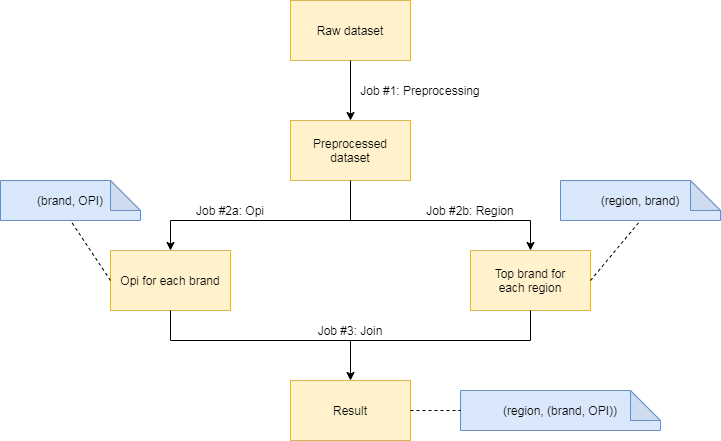
\includegraphics[scale=0.6]{images/2-mapreduce/MR-workflow.png}
	\caption{Adopted workflow for query execution.}
	\label{fig:MR-workflow}
\end{figure}

%The dataset cardinality is reduced from 423858 to 231157 * replicationFactor.
%The dataset size is reduced from 1GB to 8.2MB * replicationFactor.


